\documentclass[11pt,dvipsnames]{article}
%\usepackage[dvipdfm]{graphicx}
\usepackage{graphicx}
\usepackage{deauthor,times}
\usepackage{color}
\usepackage{xcolor}
\usepackage{xspace}
\usepackage{wrapfig}
\usepackage{enumitem}
\setlist{nosep}
\setlength{\textfloatsep}{5pt}
% The preceding line is only needed to identify funding in the first footnote. If that is unneeded, please comment it out.
\usepackage{cite}
\usepackage{amsmath,amssymb,amsfonts}
%\usepackage{hyperref}
%\usepackage{cleveref}
\usepackage{algorithmic}
\usepackage{textcomp}
\def\BibTeX{{\rm B\kern-.05em{\sc i\kern-.025em b}\kern-.08em
    T\kern-.1667em\lower.7ex\hbox{E}\kern-.125emX}}


    
\usepackage{textcomp}
\usepackage{tikz}
%\usepackage{multirow}
\usepackage{makecell, booktabs}
\usepackage{titlesec}
%\titlespacing\subsubsection{0pt}{12pt plus 4pt minus 2pt}{5pt plus 2pt minus 2pt}


\begin{document}

\title{From Cleaning before ML to Cleaning for ML}
\iffalse
\author{
  Felix Neutatz\\
  TU Berlin\\
  f.neutatz@tu-berlin.de
  \and
  Binger Chen\\
  TU Berlin\\
  chen@tu-berlin.de
  \and 
  Ziawasch Abedjan\\
  Leibniz Universit\"{a}t Hannover, \\L3S Research Center\\
  abedjan@dbs.uni-hannover.de
  \and
  Eugene Wu\\
  DSI, Columbia University\\
  ewu@cs.columbia.edu
}
\fi
\author{
  Felix Neutatz\textsuperscript{1}, Binger Chen\textsuperscript{1}, Ziawasch Abedjan\textsuperscript{2}, Eugene Wu\textsuperscript{3}\\
  \textsuperscript{1}TU Berlin, \textsuperscript{2}Leibniz Universität Hannover, \textsuperscript{2}L3S Research Center, \textsuperscript{3}DSI, \textsuperscript{3}Columbia University\\
  \{f.neutatz,chen\}@tu-berlin.de, abedjan@dbs.uni-hannover.de, ewu@cs.columbia.edu
}



\maketitle

\newcommand{\ziawasch}[1]{\textcolor{blue}{Ziawasch: #1}}
\newcommand{\Felix}[1]{\textcolor{purple}{Felix: #1}}
\newcommand{\Binger}[1]{\textcolor{red}{Binger: #1}}
\newcommand{\Eugene}[1]{\textcolor{blue}{Eugene: #1}}
\newcommand{\ewu}[1]{\textcolor{red}{ewu: #1}}
\newcommand{\todo}[1]{\textcolor{red}{TODO #1}}
%\newcommand{\stitle}[1]{\smallskip\noindent\textbf{#1}}
\newcommand{\stitle}[1]{\vspace{0.8ex}\noindent{\bf #1}}
%\newcommand{\system}{\textsc{AutoCleanML}}
%\newcommand{\system}{\textsc{QuAIitiyClean}}
\newcommand{\system}{\textsc{CycleClean}}


%modify smallest font
\newcommand{\smallestfont}{\scriptsize}



\begin{abstract}
  Data cleaning is widely regarded as a critical piece of machine learning (ML) applications, as data errors can corrupt models in ways that cause the application to operate incorrectly, unfairly, or dangerously.  
  Traditional data cleaning focuses on quality issues of a dataset in isolation of the application using the data---{\it Cleaning Before ML}---which can be inefficient and, counterintuitively, degrade the application further.    While recent cleaning approaches take into account signals from the ML model, such as the model accuracy, they are still local to a specific model, and do not take into account the entire application's semantics and user goals.
  What is needed is an end-to-end application-driven approach towards {\it Cleaning For ML}, that can leverage signals throughout the entire ML application to optimize the cleaning for application goals and to reduce manual cleaning efforts.    This paper briefly reviews recent progress in Cleaning For ML, presents our vision of a holistic cleaning framework, and outlines new challenges that arise when data cleaning meets ML applications.

\end{abstract}

%\begin{IEEEkeywords}
%component, formatting, style, styling, insert
%\end{IEEEkeywords}

\section{Introduction}

Machine learning (ML) has gained widespread adoption in real-world problems that span business~\cite{MLinTrading}, manufacturing~\cite{MLinManufacturing}, healthcare~\cite{CheXpert}, agriculture~\cite{MLinAgriculture}, and more. 
ML relies on - and is ``programmed" by - training data. Thus, the quality of the training data is a fundamental ingredient toward robust and accurate models, and ultimately toward useful and reliable ML-based applications~\cite{CleanML,Tfx,Tay}.  
For this reason, data and ML engineers spend a tremendous amount of time---80\% or more of a data scientist's time~\cite{DataCivilizer,CloudywithhighchanceofDBMS,Kandel2012EnterpriseDA}---on wrangling and cleaning the required datasets for their ML applications. 

Traditional data cleaning seeks to directly address data quality issues in a specific dataset. Given a structured dataset that potentially contains errors, it seeks to identify and/or repair those errors to derive a cleaned dataset that can be shared with the rest of the organization, or used by subsequent queries and applications without worry. Since cleaning occurs prior to, and often independent of the application, these techniques typically rely on error models to detecting duplicates or outliers, external constraint information (e.g., functional dependencies or integrity constraints), or human assessment and input (e.g., to recommend repairs or cleaning examples).  

The separation of data cleaning and the application is not optimal. For one, it is hard for users to define, or even assess, the correct integrity constraints for the application. It is also hard to anticipate the different ways that the cleaned dataset will later be used. Further, improving a dataset could in fact {\it degrade} the application~\cite{SoftwareEngineering4ML}.   Thus, it is often unclear how a given cleaning intervention will affect the downstream application. For instance, is setting an outlier value to the median the best choice for a visualization dashboard, and does it even matter?    


%\input{tables/autoML_experiments}

\begin{table}[!t]
  \centering
  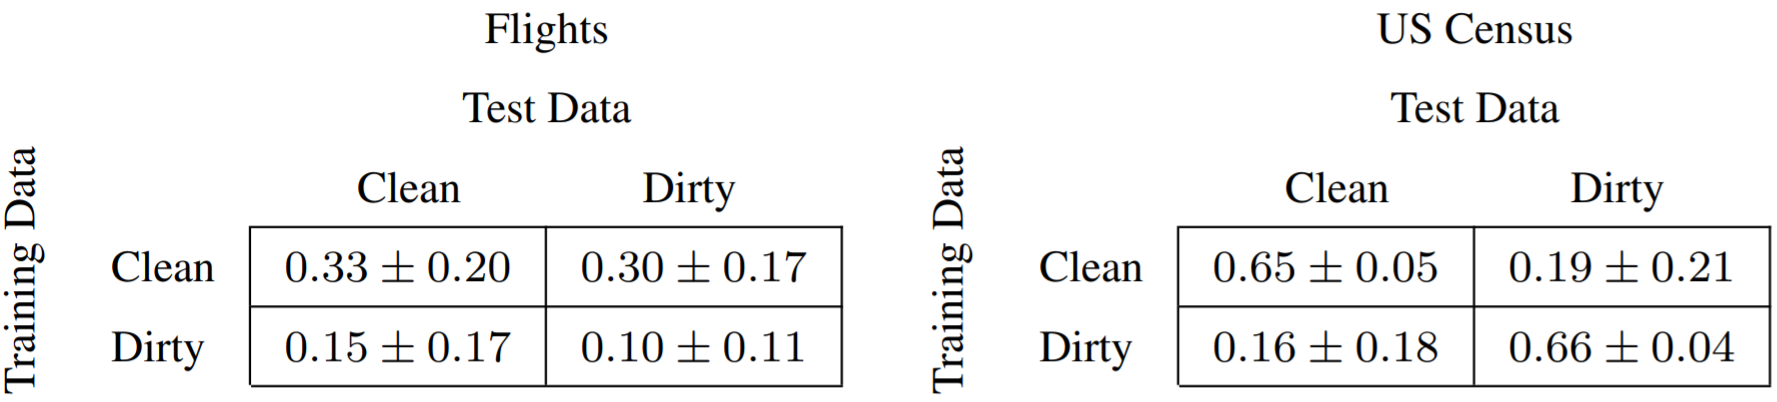
\includegraphics[width=10.9cm]{submissions/cleaning-for-ml/images/autoML.png}
  %\setlength{\abovecaptionskip}{10pt}
  \caption{Model accuracy on Flights and Census with combinations of cleaned/dirty $\times$ training/test data.}\label{fig:experiments}
\end{table}

Although these are not new issues in data cleaning, ML applications exacerbate these issues and introduce new and novel cleaning challenges. Table~\ref{fig:experiments} reports an illustrative experiment where we train a classifier using AutoSklearn~\cite{AutoSklearn} and report its accuracy on a separate test dataset.  We manually created clean and dirty versions of the FAA Flights delay~\cite{Baran} and U.S. Census~\cite{CleanML} datasets, and split each dataset using 10-fold cross-validation into training and test sets.  We find that whether or not cleaning is beneficial heavily depends on the application. For the Flights dataset, cleaned training data improves the model accuracy on both clean and dirty test data.  However, cleaning the Census training data actually degrades the model accuracy on dirty data.  In fact, training and testing on dirty data is as accurate as training and testing on clean data, yet requires no effort.    

This experiment provides evidence that cleaning is not a local ``one-and-done'' process.  In fact, \textbf{the appropriate cleaning intervention is dependent on the type of error as well as the rest of the application, and should be approached from this perspective}.    
Consequently, all of the complexities inherent in modern ML applications become complexities that affect how data is cleaned.   In this paper, we argue that data cleaning needs to take an \emph{end-to-end application-driven approach } that integrates cleaning throughout the ML application. 





\subsection{Data Cleaning in ML Applications}

\begin{wrapfigure}[11]{r}{0.47\textwidth}
	\centering
	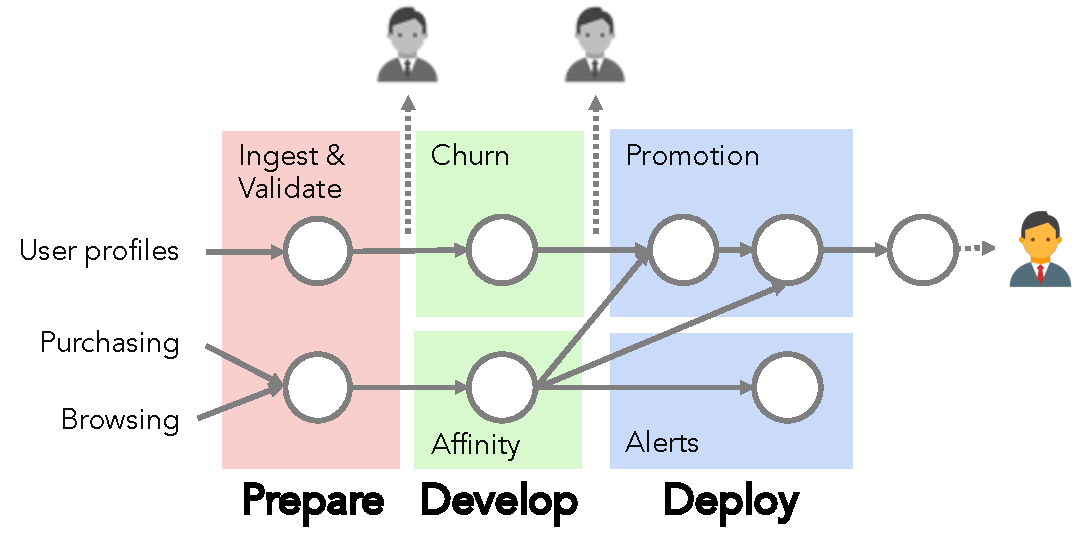
\includegraphics[width={0.47\textwidth}]{submissions/cleaning-for-ml/images/mlworkflow.pdf}
	\vspace{-2.0em}
	\caption{Typical workflow for ML applications}
	\label{f:mlworkflow}
	
\end{wrapfigure}

ML applications can be modeled as complex workflows that span an entire organization's data management, from data ingest to publishing data products to end users.    Consider an e-commerce company that identifies users for promotional discounts~(Figure~\ref{f:mlworkflow}).   The data management team ingests user profile data from a third-party data source, and combines it with internal customer purchasing and browsing histories.  The data is prepared by canonicalizing the user ids, extracting product information from the browsed pages, and ensuring that the expected attributes appear in each data record.  Separate data science teams develop two models: the first estimates the likelihood that a given user will leave the service (churn), and the second estimates a user's preference for different products (affinity).  These models are used in the promotion application to decide whether or not to show a promotion to an end-user (user in color), as well as the marketing team's internal dashboard and alert system that monitors the churn rate over time.  Different teams (colored boxes) manage different parts of the workflow, and different engineers may monitor intermediate data at different points in the workflow (dashed lines and gray users).  

\newpage%SSC
\subsubsection{Cleaning within individual phases }

The e-commerce application highlights the three prototypical phases in an ML application~\cite{MLatFacebook, Tfx}: 
the \textbf{Prepare} phase focuses on data ingestion and preparation; the \textbf{Develop} phase focuses on ML model development, training, and evaluation;  and the \textbf{Deploy} phase uses the models in the production-ready application.  Each high-level phase involves complex, multi-step data transformations and processing, and the steps are stitched together in a large workflow that often spans multiple teams within an organization.  Each phase, as well as the ML application as a whole, poses novel challenges for data cleaning.

The \textbf{Prepare} phase typically focuses on restructuring the input data so that they conform to the expected ``syntax'' of the models.  This can involve data extraction and wrangling from text documents~\cite{datawrangler}, image resizing and reshaping~\cite{ImageAugmentor}, attribute type and domain checks~\cite{Deequ,Tfx}, as well as simple constraints that any downstream application will expect~\cite{DetectingDataErrors}. There has also been a large literature on cleaning approaches that seek to address ``semantic errors''~\cite{KATARA,NADEEF,HoloClean,HoloDetect,UniDetect,MetadataDriven,Raha,ED2,Baran}.   However, most approaches do not take the subsequent workflow into account, which the above experiment showed can lead to wasted effort or even worse application outcomes.

The \textbf{Develop} phase focuses on model development, training, and evaluation.  Although the ML community has developed a multitude of robust model designs and training techniques~\cite{robustML}, it is often better to directly address errors and biases in the data~\cite{CleanML}.  Cleaning in this phase can leverage the ML models and validation data to direct cleaning efforts to most improve model quality.  In contrast to well-defined constraints that are available during the Prepare phase, quality for ML models is more challenging to define.  Using test accuracy alone is susceptible to overfitting, and other factors such as model generalization must be taken into account but are hard to quantify.   Further, ML models are often trained on nonrelational data, such as images, natural language, and unstructured documents, which require new types of cleaning interventions.

In the \textbf{Deploy} phase, trained models go into production to directly serve recommendations to end users, or as part of data analytics that power e.g., dashboards or monitoring systems. Rather than make cleaning decisions based on model quality, cleaning in this phase can leverage the ML application's user-facing results to better identify erroneous input data and save the effort of cleaning data that does not affect the output.  
However, cleaning data is harder as it may not be clear what upstream dataset (and which records) to clean, how intermediate transformations in the workflow might affect possible cleaning interventions, nor how to translate error signals into actionable interventions.  Further, external signals in this phase may override or contradict cleaning decisions made earlier in the workflow.

\subsubsection{Cleaning in ML Applications}

Stepping back, the goal of data cleaning is ultimately to improve the ML application.  This perspective presents three main challenges.  
First, the notion of data quality is more varied and often unclear. Even in traditional data cleaning, each phase has different goals: data preparation enforces syntactic constraints, model development seeks to improve model quality, while deployment seeks to improve the ML application.  Quality will often rely on a user's qualitative judgments based on application-level outputs. For instance, an analyst that examines a dashboard is well positioned to spot anomalies in the visualizations.  On the other hand, human judgments may not always be trustworthy nor correct, and attention is a limited resource.   

Second, data management, cleaning, and error detection is fragmented across different roles and different parts of the workflow.  For instance, a data management team may be responsible for data ingestion and preparation, data scientists design and train models, ML engineers then productionize and publish models that can be deployed by application developers.  At the same time, the appropriate cleaning intervention (if any is even needed) depends on the nature of the error {\it and} the model~\cite{liu_robust_2020,Zhu2020WhenDT,Diakonikolas2019SeverAR} (and application).    Thus, domain expertise is localized, visibility into the full workflow is limited, yet their cleaning decisions are conducted and felt globally.   

\newpage%SSC
Third, ML data is both complex and dynamic.  Relational, multimedia, and natural language data all require different types of interventions.  ML models are sensitive to population-level errors that can bias the model.  Further, different datasets play different roles throughout the workflow.  Ingested data is preprocessed into training data, which is distinct from test and inference data, and they are both distinct from data used for general analytics.     Finally, data constantly changes over time.  For instance, inference data today may become test or training data tomorrow.   The population-level dataset statistics, data schemas, and types of errors can change over time.  

Ultimately, data quality management in ML applications requires the ability to make informed cleaning decisions at different parts of the ML application, for different types of data and errors, and for different purposes as the data, models, and workflow evolves.  This requires coordination across the workflow so that cleaning decisions can account for downstream needs, while downstream steps can help inform upstream cleaning.   





\subsection{Looking Forward}


To this end, we propose an \emph{end-to-end application-driven approach toward cleaning}. Specifically, we envision a holistic framework that connects involved stakeholders of the entire ML application's workflow.   This framework manages the provenance of cleaning operations throughout the ML application. The provenance enables stakeholders to provide signals, cleaning suggestions, and expertise at any part of the workflow. Then, this feedback can be leveraged for cleaning in the rest of the workflow.    The framework should also
\begin{itemize}[leftmargin=*]
    \item Make it possible to change/retract cleaning decisions of early phases based on feedback obtained in later stages of the workflow; 
    \item Expose an abstract view of cleaning operations so that feedback on data quality and prior cleaning operations will be usable across all phases. Feedback on data quality will include business rules, human annotations, and the application's internal and intrinsic scores;
    \item Enable the extension and variation of the cleanliness definition in accordance with the use case at hand. It will allow for diverse error types, the weighting of errors, and error types based on importance. 
\end{itemize}

\stitle{Paper Scope:} There are two forms of data cleaning: repairing errors at the instance level (e.g., find and fix erroneous records or values), and to fix population-level errors that can arise from distributional shift, biased sampling, or record errors.  This paper primarily focuses on the former notion, and we briefly discuss population-level errors in Section~\ref{s:challenges}.



\noindent In the rest of our paper, we first review the state-of-the-art in data cleaning~(Section~\ref{sec:current}) and identify potential building blocks of our vision. Then, we layout our holistic cleaning approach and its desired component in detail. Finally, we shed light on how this vision would also address new challenges that arise in ML applications. 


\section{Data Cleaning and ML}\label{sec:current}

This section introduces and distinguishes traditional data cleaning techniques from those designed for ML.
Specifically, {\it cleaning before ML} approaches perform data cleaning independently of the downstream ML applications,
whereas {\it cleaning for ML} approaches explicitly dependent on them.


\subsection{Cleaning before ML}

Traditional data cleaning was performed during data ingestion as part of an Extract-Transform-Load (ETL) workflow.  Administrators perform data wrangling~\cite{datawrangler,potter} and transformation~\cite{DataXFormer} so that the data conforms syntactically (e.g., the appropriate schema, data types) to the application requirements.  They further specify constraints (e.g., domain constraints, functional dependency, distribution) for all database instances. The database system enforces these constraints and possibly repairs the database to address any violations.  

ML applications often combine a wide diversity of datasets, and it can be challenging for an administrator to define constraints and repair logic manually.  Thus, a number of data cleaning techniques use data-driven approaches to help detect as well as repair datasets.   The following are termed {\it Cleaning Before ML} techniques because they are primarily applied to a training dataset before model development and training, although some techniques may also be used to clean test data during model inference.   These techniques make strong assumptions about the impact of their repairs on the downstream model and application performance.  

\stitle{Non-learning Approaches.}
Data cleaning systems for error detection and/or error repair are non-learning if they directly rely on user-provided rules or specifications (which we generically term {\it cleaning signals}). 
For instance, pattern-based systems~\cite{OpenRefine,datawrangler} leverage user-specified regular expressions or patterns to identify syntactic text errors, 
while rule-based systems~\cite{NADEEF,ContinuousDataCleaning} rely on user-specified functional dependencies to identify values that violate the constraints.
Outlier detection systems~\cite{pit2016outlier,OutlierDetectionSurvey} are tuned to specific data distributions and thresholds to identify outlier values. 
Finally, systems may leverage external data such as a knowledge base~\cite{KATARA} to validate the instances of a dataset. 
For instance, if the knowledge base contains address data, KATARA can leverage it to identify mismappings between cities and ZIP codes of a given dataset.

In the context of ML applications, cleaning systems~\cite{Deequ,Tfx} help developers validate that a training set exhibits expected properties.  For instance, Deequ~\cite{Deequ} lets users declaratively write constraints, such as based on uniqueness, completeness, and value distribution, and compiles them into ``data unit-tests'' that can be executed at scale.   Many production ML platforms~\cite{Tfx,amazonvldb,Breck2019DataVF} similarly validate that training data contains expected attributes in its schema, and that data distributions have not drifted beyond a threshold.


Error repair is traditionally posed as a constraint satisfaction problem.  Given a set of data constraints, identify the minimum number of interventions so that there are no constraint violations in the dataset.  Variations of this minimality principle may include additional objectives (e.g., statistical distortion~\cite{StatisticalDistortion}), or allow a small number of violations.
The above approaches lean heavily on the user or administrator to provide accurate and useful cleaning signals, which may not always be feasible.   In addition, each approach is designed for a specific type of error, and thus exhibits low recall in practice.  ML applications may need to combine many cleaning systems to address different types of errors, or to make use of different types of cleaning signals.  We next see how learning-based cleaning seeks to address some of these limitations.



\stitle{Learning-based Approaches.}
Learning-based cleaning leverages ML to identify and repair errors.  These fall under two main directions. Ensembling approaches combine existing cleaning systems into an ensemble and use learning to decide which to use.   The alternative is to treat detection and repair as ML problems that respectively  predict whether a record is erroneous, and what the correct value for an erroneous attribute value should be.  
\vspace{3mm}
\begin{itemize}[leftmargin=*]
  \item \textbf{Error Detection: } Metadata-Driven Error Detection~\cite{MetadataDriven} and Raha~\cite{Raha} are examples of the ensembling approach, while  ED2~\cite{ED2}, DataWig~\cite{Imputation, DataWig}, HoloDetect~\cite{HoloDetect}, and Picket~\cite{Picket}.
The latter approaches model each record or cell, along with any cleaning signals, as features used to classify it as erroneous or clean.  
Naturally, learning-based approaches rely on pairs of erroneous and clean records as training examples, and semi-supervised strategies avoid the need to manually provide examples. \\

For instance, ED2~\cite{ED2} uses active learning to acquire clean/erroneous labels for records that the model is uncertain about, while Raha~\cite{Raha} further clusters records by similarity and acquires labels on a per-cluster basis.  HoloDetect~\cite{HoloDetect} uses data augmentation by learning observed error patterns and applying the patterns to generate synthetic errors.
Picket~\cite{Picket} does not rely on any external labels and instead uses self-supervision to learn an error detection model that can be applied during training or testing.  

\vspace{3mm}
\item \textbf{Error Repair: }
Repair systems such as Baran~\cite{Baran} and HoloClean~\cite{HoloClean}   combine different types of cleaning signals to more accurately repair errors.  
Baran~\cite{Baran} is an ensembling approach across a library of error repair strategies, and uses active learning to train a model that predicts which repair strategy to use.  The library of strategies is extensible, and can include additional predictive models that propose fixes. Furthermore, it uses transfer learning and label propagation to reduce the required amount of user labels.
HoloClean~\cite{HoloClean} combines integrity constraints, external data, and statistical profiles into a single factor graph model, and uses the model to predict the appropriate value for identified errors. 
\end{itemize}


\stitle{Stepping Back.}
Traditional data cleaning systems are designed around specific types of cleaning signals, whereas learning-based approaches use ensembles or models to combine a variety of signals and achieve higher recall. Weakly semi-supervised techniques such as active learning, label propagation, data augmentation, and transfer learning help reduce the degree of user involvement.  However, these approaches clean a dataset in isolation.  We next describe cleaning systems designed specifically in the context of ML applications.



\begin{table*}
\smallestfont
\centering
\caption{Taxonomy of recent cleaning for ML systems.}
\label{tab:taxonomy}
\begin{tabular}{r l l l l}
  \textbf{System}      & \textbf{Intervention Type} & \textbf{Semantics} & \textbf{Signals} & \textbf{Model Type} \\ 
ActiveClean & Manual record repair  & Model & Model Gradient  &  Convex \\ 
CPClean     & Manual value imputation & Model    & Prediction Certainties  & Nearest Neighbor \\
BoostClean  & Cleaning program        & Blackbox  & Model Validation  & Any \\
AlphaClean  & Cleaning program        & Blackbox  & Custom Objective  & Any \\
AutoSklearn & ML pipeline             & Blackbox  & Model Validation  & Any \\
Rain        & Record repairs & Relational Workflow  & User Complaint & Differentiable \\
\end{tabular}

\end{table*}



\subsection{Data Cleaning for ML}
\label{sec:sota:c4ml}

Data cleaning fundamentally relies on external cleaning signals (constraints, patterns, examples, etc.) to detect and repair data errors.   In contrast to the explicitly user-specified signals described in the previous subsection, {\it cleaning for ML} approaches leverage the downstream model or application to define cleaning signals that incorporate higher-level semantics.  This subsection describes five recent cleaning for ML systems developed in the data management community. Our rationale for this selection is that these approaches consider the semantics of the ML task and a subset of its emitted signals to deploy cleaning routines on the training dataset.
Thus, we distinguish them along four dimensions~(Table~\ref{tab:taxonomy}):
\iffalse
\begin{itemize}
  \item \stitle{Intervention Type: } whether the goal is to directly repair a dataset, or to generate a cleaning program that can be applied to future datasets as well.
  \item \stitle{Semantics: } whether the approach relies on the downstream model or application semantics, or treats it as a black box.
  \item \stitle{Signals: } the type of cleaning signal(s) that are used.
  \item \stitle{Model Type: } the type of ML models that is supported.
\end{itemize}
\fi
intervention type, semantics, signals, and model type.
The \emph{intervention type} corresponds to whether the goal is to directly repair a dataset, or to generate a cleaning program that can be applied to future datasets as well.
The \emph{semantics} describe whether the approach relies on the downstream model or application semantics, or treats it as a black box.
The \emph{signals} categorize the type of cleaning signal(s) that are used.
The \emph{model type} describes which group of ML models is supported by the corresponding approach.

\stitle{ActiveClean.}
ActiveClean~\cite{ActiveClean} is a data cleaning system for models with convex loss functions.  It treats a model trained on a dirty training set as a suboptimal point along the loss function over the (unknown) clean training set.  It then treats cleaning as a stochastic gradient descent~(SGD) problem, where in each step, the system samples and asks the user to clean records that are expected to shift the model along the steepest gradient.  The use of convex models allows the system to derive convergence guarantees.  
%
ActiveClean simply chooses which training records to repair next, but relies on the user to perform the actual repair.  Its cleaning signals combine the user's repairs and the model's loss function.  Finally, it relies on the model's convexity to guarantee convergence.   



\stitle{CPClean.}
CPClean~\cite{CPClean} incrementally cleans a training set until it is certain that no more repairs can possibly change the model predictions.  To do so, it proposes the concept of Certain Predictions~(CP) for nearest neighbor classifiers~\cite{CPClean}.  A test record is certainly predicted if all classifiers trained on all possible repairs of an incomplete training set would yield the same prediction.  CPClean develops an efficient counting query to compute the number of possible models that support a specific classification of a given test point, and uses this to quantify the impact of repairing a given error or missing value.  Thus, given a validation set, CPClean seeks to only repair the training records needed so that all validation records can be certainly predicted. 
CPClean uses the validation set and the counting query as the primary cleaning signals, but relies on the user to perform the actual repairs.   It is specially designed for nearest neighbor models, and leverages their robustness to small training perturbations.

\newpage
\stitle{BoostClean and AlphaClean.}
BoostClean~\cite{BoostClean} treats cleaning as a boosting problem, and outputs a cleaning program that can be applied to training or test records.    It is specialized to conditional value errors, where an error can be specified using a simple predicate.    Given a predefined library of parameterized detection and cleaning functions, it automatically selects a sequence of cleaning operations that will maximize the model's accuracy on a validation set (or the training set).  In each step, BoostClean uses statistical boosting to choose a pair of detection and cleaning functions and configures their parameters, and applies it to the training set to derive a new model.   BoostClean diverges from prior cleaning systems in that users do not need to manually repair records.  Instead, users simply specify appropriate detection and repair functions for the domain.  BoostClean leverages the model's training or validation accuracy as the primary cleaning signal.

AlphaClean~\cite{AlphaClean} is a similar system that generates a sequence of cleaning operations from a library of parameterized cleaning frameworks, including existing systems such as dBoost~\cite{dBoost} and HoloClean~\cite{HoloClean}.  In contrast to boosting, it uses parallelized tree search and learns pruning heuristics to reduce the search space.  Since AlphaClean uses a generic search procedure, the user is free to define their own objective function as the cleaning signal (e.g., the model accuracy, the number of constraint violations, a combination of the two).



\stitle{AutoSklearn.}
AutoSklearn~\cite{AutoSklearn} similarly uses the model validation accuracy as the primary cleaning signal to generate an end-to-end ML pipeline.  The pipeline includes preprocessing operations, hyperparameter selection, and model training.  To restrict the search space, the preprocessors are limited to value imputation based on mean, median, or most-frequent values, and are either applied to the whole dataset or not at all (e.g., no conditional repairs).    Further, AutoSklearn focuses on repairs and does not perform error detection.  




\stitle{Rain.}
Rain~\cite{ComplaintDrivenTrainingDataDebugging} seeks to go beyond an individual model and considers the downstream workflow.   It executes relational workflows consisting of relational operators and inferences made by a differentiable model.  For instance, the query ``count number of users that are likely to churn'' uses a predicate that filters by predicted churn, which is estimated by a linear regression model.     The user can annotate errors (termed ``complaints'') in the outputs or intermediate results. For instance, the user may specify that the total price in January should be 40 instead of 100, or all values in the output are too low.   Rain then ranks erroneous records (and their repairs) in the training dataset based on how much it will resolve the complaints.    
To do so, Rain models the workflow as a differentiable function over the model prediction probabilities.  The function can leverage the influence functions framework~\cite{koh2017understanding} to estimate the gradient of the query result with respect to epsilon changes to the training dataset---the removal of a training record or the addition of a new (cleaned) record.  
Their experiments show that a single annotation of an aggregate result can more effectively identify training errors than manually labeling hundreds of model mispredictions.  By supporting complaints over workflow outputs, it empowers users to specify constraints within the context of the application's downstream semantics.


\stitle{Cleaning in the ML Community.}
The ML community has long studied methods to address or circumvent data errors in learning.  
A common approach~\cite{OutlierDetectionSurvey} uses a model to classify training records as erroneous---based on model uncertainty, voting, clustering, etc---but is primarily limited to deleting records or repairing labels.
Although some errors provably require data cleaning~\cite{liu_robust_2020}, some errors can be good---training with noise is a form of regularization~\cite{bishop1995training}, and is the basis of data augmentation methods~\cite{van2001art}.  Robust estimation methods re-weigh, filter, and otherwise adapt the estimation procedure to be insensitive to outlier training data, including worst-case outliers~\cite{wilcox2011introduction,steinhardt2018robust}.  For instance, models that perform local averaging such as weighted and interpolated nearest neighbors are naturally robust to noisy training data~\cite{Belkin2018OverfittingOP}.   Models may be certified as robust to adversarial test errors~\cite{Madry2018TowardsDL,lecuyer2019certified,Raghunathan2018CertifiedDA}. The above techniques are susceptible to systematic errors.  Although they can be explicitly modeled~\cite{LearningOverDirtyDataWithoutCleaning}, this requires considerable modeling expertise, and it may not be clear what errors are even present {\it to} model. 
To this end, open source libraries such as Dabl~\cite{dabl}, Dataprep~\cite{dataprep}, and Facets~\cite{facets} combine visualization and common detection methods to aid data preparation and cleaning.




\stitle{Stepping Back.}
The database community has made significant contributions toward cleaning approaches that can be deployed in the Develop and Deploy phases. State-of-the-art cleaning for ML systems~\cite{ActiveClean, BoostClean, CPClean, AlphaClean, CPClean} leverage application-specific signals to guide human cleaning or to choose cleaning operations.
Some of them are restricted to cleaning training data and cannot generalize to unseen data~\cite{ActiveClean, CPClean}. Debugging systems, such as Rain, consider the output of an entire workflow to trace-back training instances that lead to wrong results. 
A recurrent problem is that each proposed solution only covers a specific aspect of cleaning, such as specific error types, dataset components, or ML models. As a result, a successful attempt at cleaning a dataset for deployment forces analysts and scientists to use multiple disconnected approaches.



\section{Cleaning for ML Applications}\label{sec:vison}

The Introduction highlighted three major challenges toward data cleaning for ML applications.
First, the definition of data quality and what a data error even means is not only user-defined, but is also model- and application-specific.  This makes these definitions difficult to foresee and articulate during the model design and data ingestion phase.
Second, domain knowledge and expertise is fragmented across the different users---developers, ML experts, IT staff, and end users---that each have limited visibility into the ML application's workflow (or workflow for short).
Third, ML applications are complex, dynamic, and heterogeneous.  They combine and process relational and non-relational data streams whose properties may continuously change over time.  

As a step toward tackling these challenges, this section describes a research agenda that extends data cleaning to encompass the needs of ML applications.  
We first center the agenda around a high-level architecture, and then highlight a number of promising research challenges in each of the architectural components.

\subsection{Architecture}

\begin{wrapfigure}{r}{0.46\textwidth}
	\centering
	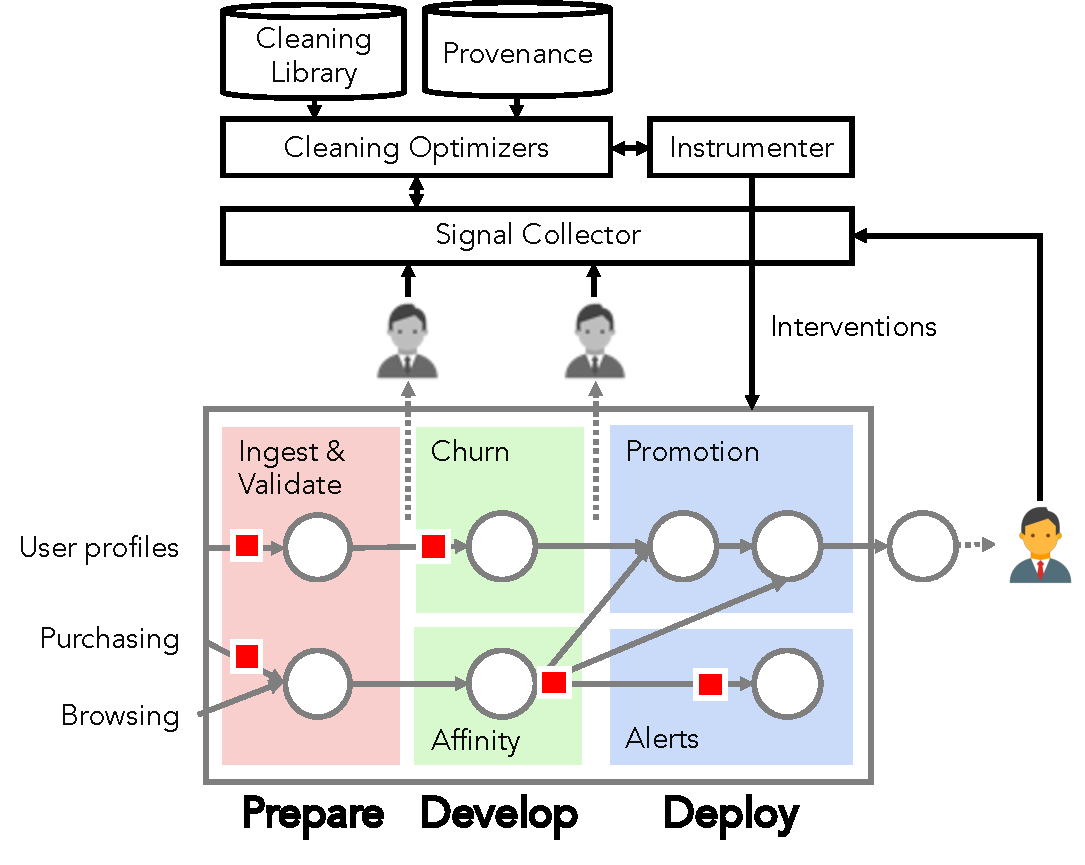
\includegraphics[width={0.45\textwidth}]{submissions/cleaning-for-ml/images/arch-1-17.pdf}
	\caption{Envisioned Holistic Cleaning Framework.}
	\label{figure:workflow}
	%\vspace{-1.0em}
\end{wrapfigure}
Data cleaning is fundamentally human-centered.  Humans design the ML application with specific goals in mind; humans build, operate, and maintain each component of the application's workflow; and humans use the resulting application to accomplish their tasks.  Thus, it is crucial to ``bring cleaning to the user.''  At any point in the workflow, it should be easy to inspect the data that flows through, and provide data quality signals that help to make error detection and repair decisions.

We envision data cleaning as an instrumentation layer that sits atop the entire application workflow~(Figure~\ref{figure:workflow}).  Its purpose is to use elicit cleaning signals throughout the workflow to decide which data to clean, how to improve data quality, and where in the workflow to instrument which cleaning operations.    
%
The dashed lines denote workflow steps that serve as inspection points for users and provide cleaning signals to the {\it Signal Collector}. The inspected data can first be processed and transformed (e.g., by a script or query) before being rendered to the user (e.g., as a table, interactive visualization).  The key characteristic of any data interface is that it can be annotated with data errors that the user sees, expected trends or data properties, or any other signal that can aid the cleaning system.  These signals are collected and routed to {\it Cleaning Optimizers} that make local or global cleaning decisions about what cleaning operations to install or test. The {\it Instrumenter} then augments the workflow with cleaning operations (red squares), and monitors their effectiveness over time.  The monitoring signals serve as additional feedback to improve the optimizers.  
The user input-optimize-clean loop is a classic approach toward user-centered data cleaning~\cite{End2EndHumanCentricCleaning}.  The key distinction of the proposed design is that this loop permeates throughout the ML application.   Data that is deeper in the workflow encodes increasingly more application semantics and qualitatively changes the scope and type of cleaning signals that users can provide.   For instance, signals collected during the Develop phase can leverage model-specific statistics to quantify data quality, while signals in the Deploy phase, such as data presented to the end user, encode utility toward the user's task. This parallels visual analytics, which transforms, filters, and summarizes data as visualizations to surface unanticipated trends and patterns that are not visible, nor easily expressible, in the raw data. 

\subsection{Signal Collection}

Cleaning signals are external information that initiate and inform data cleaning in the workflow.  Existing cleaning approaches assume a single cleaning signal is collected at a specific point in the workflow, and is coupled with the cleaning algorithm (Section~\ref{sec:sota:c4ml}).  In contrast, we envision a framework that can request and collect cleaning signals from any point in the workflow at varying levels of applicaton abstractions. 

\subsubsection{Signal Types}

In general, a cleaning signal is any information that can aid data cleaning.  Signals can be provided by the users (e.g., through a visualization), derived from the application (e.g., model accuracy), or programmatically generated (e.g., an alert, or constraint violation).
We initially propose to support the four types of signals---constraints, rules, annotations, and objectives---commonly used in existing cleaning systems.   

Integrity constraints~\cite{NADEEF}, such as functional dependencies, denial constraints, can be specified for any input, intermediate, or output dataset in the workflow.  They can be used directly, or be used to trigger alert signals when they detect violations.  
Similarly, ML-specific constraints may specify e.g., fairness~\cite{InterventionalFairness}, robustness, or generalization properties.
Constraints may be user-specified or automatically generated.

Rules include predicates to remove records or ETL transformations, and may trigger signals when they fail.  
Manual annotations of a dataset specify erroneous records or values.  For instance, a user may annotate that a value should be 50 instead of 30, or provide a label for a training record.   
Annotations can also be automatically computed in the workflow through application-specific scores, such as the model validation score~\cite{BoostClean, AutoSklearn, AlphaClean}, prediction certainty~\cite{CPClean}, and gradient information~\cite{ActiveClean}.
Finally, the cleaning system can directly listen on the actual application objective, such as classification accuracy.



\subsubsection{Eliciting Signals}
To elicit the various user and application-specific signals from the ML workflow, it must be possible for the cleaning system to inspect workflow data. This leads to two main questions:

\stitle{Where to elicit?}  When used as part of data debugging or engineering, there are natural points in the workflow where users are accustomed to provide signals.  These typically include data ingestion, before and after model training, and the application output. However,  there are likely other useful points to assess data quality to detect potential errors, or to elicit signals to aid later cleaning.  For instance, it is often difficult to coordinate across organizations, thus collecting signals at steps that cross organizational boundaries may be prudent.

A major research question is what signals should be elicited during data cleaning.  Once a user has reported a data error (say, in the application output), where should additional signals be collected that can improve the cleaning algorithms?  For instance, the algorithm may generate candidate repairs and ask the user to label them; or ask users to annotate other application outputs to choose between possible repairs; or ask for integrity constraints to narrow a search space.    This is also an opportunity to automatically collect signals (e.g., model accuracies) without any user effort. 


\newpage
\stitle{What elicitation interfaces?} 
Users should be able to use interfaces to interactively e.g., confirm or highlight errors in the data~\cite{ED2, Raha, Baran}, provide example records~\cite{Baran,DataXFormer}, and specify constraints or rules~\cite{NADEEF}.    Assuming that workflow data is structured, an initial approach is to provide a library of general data presentation options, such as automatic data visualization~\cite{apt,ShowMe}, spreadsheet interfaces, or a scripting environment.  
Further, systems can interactively explain error causes and how they are detected/corrected~\cite{DataXRay, Scorpion, CAPE_OutlierExplanation, BugDoc, Vizier, ReverseDataManagement}.
Here, one research opportunity is to design recommender systems that propose the best setup from a large number of potential visualization methods based on previous user interaction and metadata. Collecting signals at these various phases enables to clean training, test, and deployment data with the same cleaning goals in mind to avoid distributional gaps.

\subsection{Cleaning Optimizers}

Signals represent the application or user's expectations about data quality, and can be both used to initiate data cleaning or improve cleaning quality.  For instance, a user annotation may notice an output error, which triggers the need to cleaning a training dataset; an integrity constraint on the training data helps prune the algorithm's search space since it is already enforced.     
%
The purpose of the cleaning optimizer is to combine different signals and propose a pipeline of cleaning operations that detect and repair errors in a dataset, and where to apply them. 
Each cleaning optimizer may be an existing signal-specific cleaning system (such as those in Section~\ref{sec:current}) or new ``holistic'' optimizers that combine disparate signals.  Each optimizer should specify the subset of the workflow it can be responsible for (e.g., model training, data preparation, relational sub-workflows), the signal types it requests, and crucially, the types of interventions it accounts for.   
%
We distinguish optimizers along two dimensions: whether the optimizer is local to a phase or operator in the workflow, or takes a subset or whole workflow into account; and whether the optimizer treats the workflow as a white or black box.  


\subsubsection{A ``Holistic'' Cleaning Optimizer}
An open question is to what extent different signals throughout the workflow can be integrated to holistically clean data in the workflow.  The different signal types naturally express hard  constraints, soft constraints, and objective functions, thus may be amenable toward translating into a singular optimization problem.  Prior works such as HoloClean~\cite{HoloClean} and Baran~\cite{Baran} have shown how this is possible using factor graphs and ensembles for specific combinations of signals.  Many existing works focus on specific classes of data errors, signals, and workflows, and a major challenge is how to support a wider range of signal types, interventions, different collection points, and incorporating the workflow semantics.  


\subsubsection{Workflow-independent vs -dependent Optimizers}
A workflow-independent optimizer is specific to a single workflow operator and does not use any workflow semantics.  Most existing systems that clean~\cite{HoloClean,NADEEF}, wrangle~\cite{datawrangler,NADEEF,OpenRefine}, or transform~\cite{DataXFormer} a specific dataset are workflow-independent. 
In contrast, a workflow-dependent optimizer cleans data at a given point in the workflow by using signals (e.g., model accuracy, user annotations) from downstream and/or upstream.   Although recent cleaning systems incorporate downstream signals~\cite{BoostClean,AlphaClean,CPClean,AutoSklearn}, it is an open question how to integrate multiple cleaning signals collected from different points in the workflow and optimize in a workflow-dependent manner.


\subsubsection{White vs Black Box}

Workflow-dependent optimizers combine workflow semantics and cleaning signals.  For instance, if a user specifies errors in the application output, and the system wishes to clean ingested data during the Prepare phase, it needs to consider all of the workflow's operator semantics to assess how different cleaning decisions would affect the output.  
Optimizers can be either implemented as a white or black-box approach. 

In white-box approaches, the optimizer has access to signals of every single transformation in the ML pipeline, and leverages well-defined workflow semantics (e.g., in relational workflows) to encode the pipeline logic into constraints and/or an optimization objective. For instance, Rain encodes the SQL query as a relaxed provenance polynomial, and can evaluate custom record-level interventions.
A white-box-specific optimization is to reduce the overhead of retraining by avoiding repetitive computation through partial retraining~\cite{DeltaGrad,IncrementallyUpdatingRegression} or caching~\cite{Helix, SystemDS}.

In contrast, black-box approaches ignore intermediate results and simply reason about the workflow input and output.  They may translate cleaning signals into optimization constraints and objectives, and use generic black-box optimization techniques such as meta-learning techniques or Bayesian optimization to search the space of cleaning interventions. Existing meta-learning approaches that ensemble many cleaning algorithms (e.g., Raha~\cite{Raha}, Baran~\cite{Baran}) only encode dataset properties in their feature vector and ignore the semantics of the application workflow.  BOExplain~\cite{boexplain} treats workflow cleaning as a blackbox hyperparameter search problem.
Ultimately, the key challenge is to define an effective but concise search space, and to create a workflow representation that facilitates meta learning for ML-dependent cleaning. 


White-box approaches can be more accurate and efficient, but do not readily support custom logic or user-defined functions.  
On the other hand, black-box approaches can be applied to any ML workflow, but can be very inefficient.  
A potential middle-ground is to approximate the workflow using heuristics, or making assumptions about the workflow operator semantics.   For instance, the system might approximate an operator using an ML model~\cite{CPClean}, or symbolically execute the operator to derive a logical expression~\cite{Froid,Acorn}.  
Another interesting direction is to trace back the error causes to the corresponding workflow components~\cite{DataXRay}. 



\subsection{Scope Refinement}

When there are many data sources, datasets, and annotations, a fundamentally challenging problem is knowing which datasets are the candidates that may be responsible for the annotations. We call this the {\it Scope} of the annotations.  There are several promising directions for scope refinement.

One approach to identify the datasets to clean is to assess their potential impact on the error annotations, either directly using sensitivity analysis~\cite{ComplaintDrivenTrainingDataDebugging}, or using a framework akin to certain predictions~\cite{CPClean}. Assuming that the dataset to clean is known, one way to refine scope is to use feature~\cite{FeatureSelection} or instance selection~\cite{InstanceSelection} to identify the most important columns and rows in the training data. ActiveClean and CPClean follow the instance selection approach~\cite{ActiveClean,CPClean}.
A third direction is to narrow the scope to the provenance of the annotated data~\cite{ComplaintDrivenTrainingDataDebugging}.  However, this can still be a large set of records.  For instance, the end-user-facing output of the ML applications trivially depends on all of the datasets (and a subset of their records).  

Research opportunities in this field are to combine workflow-dependent optimization with scope refining strategies. The optimizer could generate different cleaning pipelines for different scopes of the data. For example, it could generate a set of cleaning operations based on functional dependencies for categorical data and use a Gaussian outlier detection technique and use a ``replace with median value'' as the default cleaning operation for numerical features. Some cleaning pipelines might be more general and cover a larger scope of the dataset leading to unnecessary cleaning efforts but instrumenting individual pipelines, which are simpler, for specific subsets of the dataset might introduce an unnecessary overhead. Automatically identifying the best scope refinement and the best trade-off for a dataset at hand is an interesting research problem. 
Being able to distinguish different scopes of a dataset also enables to prioritize cleaning efforts for the most significant scopes. Thus, one can decide to instrument cleaning on dataset subsets that are small but significant to speed-up real-time model and configuration testing in the Develop phase. 


\subsection{Instrumenter}

Once the cleaning optimizers have chosen promising interventions, they need to be instrumented into the workflow.  Although most systems support dynamic instrumentation, it alone is not sufficient, as the workflow and the data properties may differ from the assumptions made during optimization, and can also change over time.
In real-world applications, data constantly changes over time~\cite{SergeysPaper,ContinuousDataCleaning, ValidationforDynamicDataIngestion}. The challenge is to identify when the distribution shifted too much so that any of the installed cleaning rules do not apply anymore.
Thus, it is crucial to provide assessment and monitoring functionalities to aid the engineers to manage the data cleaning process.


One can investigate how to backtest or speculatively test interventions before installing them. Another interesting direction is to define an algorithm that periodically or continuously assesses the effectiveness of past cleaning interventions.
Ultimately, the monitoring approach helps the data cleaning ``team'' to manage the disparate cleaning signals collected throughout the workflow to understand which are reliable, are consistent with each other, and which are used for a given intervention. A practical challenge here is to efficiently keep track of instrumented cleaning operations and data changes. Existing approaches that ensemble cleaning operators have to keep track of thousands of operators~\cite{Raha,Baran} on each dataset. One could think of index-based solutions to scale the trace-back requests for large datasets or develop models that learn and predict the relationships. 



\section{New Challenges of Cleaning for ML}\label{s:challenges}
The previous section outlined our vision of holistic and flexible data cleaning for ML applications, and research opportunities related to the different components. 

Data cleaning systems, including the proposed system in this paper, have historically been designed for structured, e.g., relational,  and persistent datasets. Within this scope, they have focused on record and value-level errors, and data quality metrics are designed for these errors in mind, e.g., number of constraint violations, outlier-ness of a value.  
However, there are a number of challenges that go beyond the scope of our proposed vision.
The type of input data used in ML workflows goes beyond structured data and can become less tangible through entanglement of models. 

The notion of data quality is also much broader in scope for ML applications, and includes population-level errors, as well as social and cultural norms. This subsection describes these novel challenges and provides pointers for further consideration.



\stitle{Unstructured data.} ML approaches are especially successful for unstructured data, such as images, sound, and video. Traditional data management cleaning approaches and their cleaning operations focus on numeric, categorical, and textual data~\cite{ED2, Raha, Baran, HoloClean, HoloDetect}.  The proliferation of generative models offers the potential to similarly repair unstructured data by transforming e.g., images in semantically meaningful ways.

\stitle{Model entanglement.} This phenomenon arises when a model (or a component in general) compensates for errors in an upstream model~\cite{SoftwareEngineering4ML,HiddenTechnicalDebt}.   In this setting, the models are entangled, and improving any model individually will degrade the end-to-end performance.  In general, hidden dependencies across different parts of the application can severely complicate data cleaning, and necessitates the need to incorporate downstream signals and workflow logic into the cleaning process.   Identifying and disassociating entangled components is another important problem to tackle. 

\stitle{Population-level Errors:}  This paper focused on record-level errors, however population-level errors also impact ML applications today.  These may be due to biased sampling, or systematic errors from data generating processes or preprocessing logic, and manifest as biased models and biased predictions.  In these contexts, even cleaning all of the records in a dataset may not fully address the distributional biases.  These errors can affect the ML application in not just biased predictions---differences between training and test distributions, or distribution drift over time can all introduce application-level issues.  

Although there is work in detecting distributional shifts in a dataset~\cite{lipton2018detecting,abdelkader2020towards}, accounting for group-wise errors (and interventions) the downstream implications is considerably more challenging than doing so for an individual record due to interaction effects~\cite{Koh2019OnTA}. Furthermore, continuing the research on pre-processing techniques~\cite{InterventionalFairness} to avoid bias and inspecting pipelines for violating data patterns~\cite{Grafbergercidr2021} is a promising direction to explore.

\stitle{Social/cultural norms:} Another new generation of errors are violations against social and cultural norms. For instance, one should avoid training on text, image, sound, or video corpora that contain hate speech~\cite{Tay}, misinformation~\cite{Scrutinizer}, or privacy violations~\cite{ExtractingTrainingDatafromLanguageModels, Amnesia}. While some of these issues could be identified with lists of forbidden words, many might not be initially obvious to a human. The problems might appear in the downstream application in a more tangible form, which motivates to design algorithms that can trace the results back to data. These re-emerging quality dimensions are also changing over time. A potential direction is to design active-learning systems that support users to continuously define these norms.

\stitle{Robustness Prediction:} An increasingly important field in ML is safety~\cite{Picket}.  Out-of-distribution~\cite{lee_simple_nodate} or adversarial test records can cause the ML model to make wrong predictions. ML-driven cleaning has the potential to help tackle these issues.  Although individual value errors may be hard to detect, identifying erroneous records with respect to the model or application may be possible.  

\stitle{Clever Hans.}  
The ML pipeline is expected to work well (to generalize) on new unseen data---training data used to update models, data used to make predictions, or any other data used in the application. Guiding the cleaning efforts with signals, such as validation score or uncertainty, might mislead the cleaning efforts through spurious correlations~(Clever Hans phenomenon~\cite{CleverHans}). While in the Develop phase the cleaning might lead to higher accuracy, because it used the spurious correlations, we might end up with lower performance because these correlations are not prevalent. E.g., Lapuschkin et al.~\cite{CleverHans} found that their trained ML model used the source tag~\emph{horse\_photo\_archive.de} to classify images as horses instead of actual horse characteristics, such as its tail or its head. While the model performed very well on that dataset, it clearly missed the goal of capturing the visual features of a horse. Cleaning that is guided by accuracy might aggravate this problem. To prevent Clever Hans phenomena, it is not enough to have a feedback loop from the Deploy phase. A promising direction is to make model explanation an integral part of data cleaning. 



\section*{Acknowledgments}

This work was funded by the German Ministry for Education and Research as BIFOLD - Berlin Institute for the Foundations of Learning and Data (ref. 01IS18025A and ref. 01IS18037A); Eugene Wu was funded by National Science Foundation awards 1564049, 1845638, and 2008295, Amazon and Google research awards, and a Columbia SIRS award.  


%\bibliographystyle{IEEEtran}
%\bibliography{abbreviations}

% Generated by IEEEtran.bst, version: 1.14 (2015/08/26)
\providecommand{\noopsort}[1]{}
\begin{thebibliography}{10}
\providecommand{\url}[1]{#1}
\csname url@samestyle\endcsname
\providecommand{\newblock}{\relax}
\providecommand{\bibinfo}[2]{#2}
\providecommand{\BIBentrySTDinterwordspacing}{\spaceskip=0pt\relax}
\providecommand{\BIBentryALTinterwordstretchfactor}{4}
\providecommand{\BIBentryALTinterwordspacing}{\spaceskip=\fontdimen2\font plus
\BIBentryALTinterwordstretchfactor\fontdimen3\font minus
  \fontdimen4\font\relax}
\providecommand{\BIBforeignlanguage}[2]{{%
\expandafter\ifx\csname l@#1\endcsname\relax
\typeout{** WARNING: IEEEtran.bst: No hyphenation pattern has been}%
\typeout{** loaded for the language `#1'. Using the pattern for}%
\typeout{** the default language instead.}%
\else
\language=\csname l@#1\endcsname
\fi
#2}}
\providecommand{\BIBdecl}{\relax}
\BIBdecl

\bibitem{MLinTrading}
Y.~Deng, F.~Bao, Y.~Kong, Z.~Ren, and Q.~Dai, ``Deep direct reinforcement
  learning for financial signal representation and trading,'' \emph{{IEEE}
  Trans. Neural Networks Learn. Syst.}, vol.~28, no.~3, pp. 653--664, 2017.

\bibitem{MLinManufacturing}
P.~Priore, D.~de~la Fuente, A.~G{\'{o}}mez, and J.~Puente, ``A review of
  machine learning in dynamic scheduling of flexible manufacturing systems,''
  \emph{Artif. Intell. Eng. Des. Anal. Manuf.}, vol.~15, no.~3, pp. 251--263,
  2001.

\bibitem{CheXpert}
J.~Irvin, P.~Rajpurkar, M.~Ko, Y.~Yu, S.~Ciurea{-}Ilcus, C.~Chute, H.~Marklund,
  B.~Haghgoo, R.~L. Ball, K.~S. Shpanskaya, J.~Seekins, D.~A. Mong, S.~S.
  Halabi, J.~K. Sandberg, R.~Jones, D.~B. Larson, C.~P. Langlotz, B.~N. Patel,
  M.~P. Lungren, and A.~Y. Ng, ``Che{X}pert: {A} large chest radiograph dataset
  with uncertainty labels and expert comparison,'' in \emph{AAAI}, 2019, pp.
  590--597.

\bibitem{MLinAgriculture}
K.~Liakos, P.~Busato, D.~Moshou, S.~Pearson, and D.~Bochtis, ``Machine learning
  in agriculture: {A} review,'' \emph{Sensors}, vol.~18, no.~8, p. 2674, 2018.

\bibitem{CleanML}
P.~Li, X.~Rao, J.~Blase, Y.~Zhang, X.~Chu, and C.~Zhang, ``{CleanML:} a study
  for evaluating the impact of data cleaning on ml classification tasks,'' in
  \emph{ICDE}, 2021.

\bibitem{Tfx}
D.~Baylor, E.~Breck, H.-T. Cheng, N.~Fiedel, C.~Y. Foo, Z.~Haque, S.~Haykal,
  M.~Ispir, V.~Jain, L.~Koc \emph{et~al.}, ``Tfx: A tensorflow-based
  production-scale machine learning platform,'' in \emph{SIGKDD}, 2017, pp.
  1387--1395.

\bibitem{Tay}
\BIBentryALTinterwordspacing
P.~Lee. (2016) Learning from {Tays} introduction. [Online]. Available:
  \url{https://blogs.microsoft.com/blog/2016/03/25/learning-tays-introduction/}
\BIBentrySTDinterwordspacing

\bibitem{DataCivilizer}
D.~Deng, R.~C. Fernandez, Z.~Abedjan, S.~Wang, M.~Stonebraker, A.~K.
  Elmagarmid, I.~F. Ilyas, S.~Madden, M.~Ouzzani, and N.~Tang, ``The data
  civilizer system,'' in \emph{CIDR}, 2017.

\bibitem{CloudywithhighchanceofDBMS}
A.~Agrawal, R.~Chatterjee, C.~Curino, A.~Floratou, N.~Godwal, M.~Interlandi,
  A.~Jindal, K.~Karanasos, S.~Krishnan, B.~Kroth, J.~Leeka, K.~Park, H.~Patel,
  O.~Poppe, F.~Psallidas, R.~Ramakrishnan, A.~Roy, K.~Saur, R.~Sen, M.~Weimer,
  T.~Wright, and Y.~Zhu, ``Cloudy with high chance of {DBMS:} a 10-year
  prediction for enterprise-grade {ML},'' in \emph{CIDR}, 2020.

\bibitem{Kandel2012EnterpriseDA}
S.~Kandel, A.~Paepcke, J.~M. Hellerstein, and J.~Heer, ``Enterprise data
  analysis and visualization: An interview study,'' \emph{TVCG}, vol.~18, pp.
  2917--2926, 2012.

\bibitem{SoftwareEngineering4ML}
S.~Amershi, A.~Begel, C.~Bird, R.~DeLine, H.~C. Gall, E.~Kamar, N.~Nagappan,
  B.~Nushi, and T.~Zimmermann, ``Software engineering for machine learning: a
  case study,'' in \emph{ICSE}, 2019, pp. 291--300.

\bibitem{AutoSklearn}
M.~Feurer, A.~Klein, K.~Eggensperger, J.~T. Springenberg, M.~Blum, and
  F.~Hutter, ``Efficient and robust automated machine learning,'' in
  \emph{NeurIPS}, 2015, pp. 2962--2970.

\bibitem{Baran}
M.~Mahdavi and Z.~Abedjan, ``Baran: Effective error correction via a unified
  context representation and transfer learning,'' \emph{PVLDB}, vol.~13,
  no.~11, pp. 1948--1961, 2020.

\bibitem{MLatFacebook}
K.~M. Hazelwood, S.~Bird, D.~M. Brooks, S.~Chintala, U.~Diril, D.~Dzhulgakov,
  M.~Fawzy, B.~Jia, Y.~Jia, A.~Kalro, J.~Law, K.~Lee, J.~Lu, P.~Noordhuis,
  M.~Smelyanskiy, L.~Xiong, and X.~Wang, ``Applied machine learning at
  {F}acebook: {A} datacenter infrastructure perspective,'' in \emph{HPCA},
  2018, pp. 620--629.

\bibitem{datawrangler}
S.~Kandel, A.~Paepcke, J.~M. Hellerstein, and J.~Heer, ``Wrangler: interactive
  visual specification of data transformation scripts,'' in \emph{CHI}, 2011,
  pp. 3363--3372.

\bibitem{ImageAugmentor}
M.~D. Bloice, C.~Stocker, and A.~Holzinger, ``Augmentor: An image augmentation
  library for machine learning,'' \emph{J. Open Source Softw.}, vol.~2, no.~19,
  p. 432, 2017.

\bibitem{Deequ}
S.~Schelter, F.~Bie{\ss}mann, D.~Lange, T.~Rukat, P.~Schmidt, S.~Seufert,
  P.~Brunelle, and A.~Taptunov, ``Unit testing data with deequ,'' in
  \emph{SIGMOD}, 2019, pp. 1993--1996.

\bibitem{DetectingDataErrors}
Z.~Abedjan, X.~Chu, D.~Deng, R.~C. Fernandez, I.~F. Ilyas, M.~Ouzzani,
  P.~Papotti, M.~Stonebraker, and N.~Tang, ``Detecting data errors: Where are
  we and what needs to be done?'' \emph{PVLDB}, vol.~9, no.~12, pp. 993--1004,
  2016.

\bibitem{KATARA}
X.~Chu, J.~Morcos, I.~F. Ilyas, M.~Ouzzani, P.~Papotti, N.~Tang, and Y.~Ye,
  ``{KATARA:} {A} data cleaning system powered by knowledge bases and
  crowdsourcing,'' in \emph{SIGMOD}, 2015, pp. 1247--1261.

\bibitem{NADEEF}
M.~Dallachiesa, A.~Ebaid, A.~Eldawy, A.~K. Elmagarmid, I.~F. Ilyas, M.~Ouzzani,
  and N.~Tang, ``{NADEEF:} a commodity data cleaning system,'' in
  \emph{SIGMOD}, 2013, pp. 541--552.

\bibitem{HoloClean}
T.~Rekatsinas, X.~Chu, I.~F. Ilyas, and C.~R{\'{e}}, ``{HoloClean:} holistic
  data repairs with probabilistic inference,'' \emph{PVLDB}, vol.~10, no.~11,
  pp. 1190--1201, 2017.

\bibitem{HoloDetect}
A.~Heidari, J.~McGrath, I.~F. Ilyas, and T.~Rekatsinas, ``{HoloDetect:}
  few-shot learning for error detection,'' in \emph{SIGMOD}, 2019, pp.
  829--846.

\bibitem{UniDetect}
P.~Wang and Y.~He, ``{Uni-Detect:} {A} unified approach to automated error
  detection in tables,'' in \emph{SIGMOD}, 2019, pp. 811--828.

\bibitem{MetadataDriven}
L.~Visengeriyeva and Z.~Abedjan, ``Metadata-driven error detection,'' in
  \emph{SSDBM}, 2018, pp. 1:1--1:12.

\bibitem{Raha}
M.~Mahdavi, Z.~Abedjan, R.~C. Fernandez, S.~Madden, M.~Ouzzani, M.~Stonebraker,
  and N.~Tang, ``Raha: {A} configuration-free error detection system,'' in
  \emph{SIGMOD}, 2019, pp. 865--882.

\bibitem{ED2}
F.~Neutatz, M.~Mahdavi, and Z.~Abedjan, ``{ED2:} {A} case for active learning
  in error detection,'' in \emph{CIKM}, 2019, pp. 2249--2252.

\bibitem{robustML}
J.~Z. Li, ``Principled approaches to robust machine learning and beyond,''
  Ph.D. dissertation, Massachusetts Institute of Technology, Cambridge, {USA},
  2018.

\bibitem{liu_robust_2020}
Z.~Liu, J.~Park, N.~Palumbo, T.~Rekatsinas, and C.~Tzamos, ``Robust {Mean}
  {Estimation} under {Coordinate}-level {Corruption} with {Missing}
  {Entries},'' \emph{arXiv}, 2020.

\bibitem{Zhu2020WhenDT}
B.~Zhu, J.~Jiao, and J.~Steinhardt, ``When does the tukey median work?''
  \emph{ISIT}, pp. 1201--1206, 2020.

\bibitem{Diakonikolas2019SeverAR}
I.~Diakonikolas, G.~Kamath, D.~Kane, J.~Li, J.~Steinhardt, and A.~Stewart,
  ``Sever: A robust meta-algorithm for stochastic optimization,'' in
  \emph{ICML}, 2019.

\bibitem{potter}
V.~Raman and J.~M. Hellerstein, ``Potter's wheel: An interactive data cleaning
  system,'' in \emph{VLDB}, 2001, pp. 381--390.

\bibitem{DataXFormer}
Z.~Abedjan, J.~Morcos, I.~F. Ilyas, M.~Ouzzani, P.~Papotti, and M.~Stonebraker,
  ``Dataxformer: {A} robust transformation discovery system,'' in \emph{ICDE},
  2016, pp. 1134--1145.

\bibitem{OpenRefine}
\BIBentryALTinterwordspacing
(2021) Open{R}efine. [Online]. Available: \url{https://openrefine.org/}
\BIBentrySTDinterwordspacing

\bibitem{ContinuousDataCleaning}
M.~Volkovs, F.~Chiang, J.~Szlichta, and R.~J. Miller, ``Continuous data
  cleaning,'' in \emph{ICDE}, 2014, pp. 244--255.

\bibitem{pit2016outlier}
C.~Pit-Claudel \emph{et~al.}, ``Outlier detection in heterogeneous datasets
  using automatic tuple expansion,'' Technical Report MIT-CSAIL-TR-2016-002,
  CSAIL, MIT, 32 Vassar Street, Cambridge MA 02139, Tech. Rep., 2016.

\bibitem{OutlierDetectionSurvey}
V.~J. Hodge and J.~Austin, ``A survey of outlier detection methodologies,''
  \emph{Artif. Intell. Rev.}, vol.~22, no.~2, pp. 85--126, 2004.

\bibitem{amazonvldb}
S.~Schelter, D.~Lange, P.~Schmidt, M.~Celikel, F.~Bie{\ss}mann, and
  A.~Grafberger, ``Automating large-scale data quality verification,''
  \emph{{PVLDB}}, vol.~11, no.~12, pp. 1781--1794, 2018.

\bibitem{Breck2019DataVF}
E.~Breck, N.~Polyzotis, S.~Roy, S.~Whang, and M.~Zinkevich, ``Data validation
  for machine learning,'' in \emph{MLSys}, 2019.

\bibitem{StatisticalDistortion}
T.~Dasu and J.~M. Loh, ``Statistical distortion: Consequences of data
  cleaning,'' \emph{PVLDB}, vol.~5, no.~11, pp. 1674--1683, 2012.

\bibitem{Imputation}
F.~Bie{\ss}mann, D.~Salinas, S.~Schelter, P.~Schmidt, and D.~Lange, ``"{D}eep"
  learning for missing value imputation in tables with non-numerical data,'' in
  \emph{CIKM}, 2018, pp. 2017--2025.

\bibitem{DataWig}
F.~Bie{\ss}mann, T.~Rukat, P.~Schmidt, P.~Naidu, S.~Schelter, A.~Taptunov,
  D.~Lange, and D.~Salinas, ``Data{W}ig: Missing value imputation for tables,''
  \emph{J. Mach. Learn. Res.}, vol.~20, pp. 175:1--175:6, 2019.

\bibitem{Picket}
Z.~Liu, Z.~Zhou, and T.~Rekatsinas, ``Picket: Self-supervised data diagnostics
  for {ML} pipelines,'' \emph{CoRR}, vol. abs/2006.04730, 2020.

\bibitem{ActiveClean}
S.~Krishnan, J.~Wang, E.~Wu, M.~J. Franklin, and K.~Goldberg, ``{ActiveClean:}
  interactive data cleaning for statistical modeling,'' \emph{PVLDB}, vol.~9,
  no.~12, pp. 948--959, 2016.

\bibitem{CPClean}
B.~Karlas, P.~Li, R.~Wu, N.~M. G{\"{u}}rel, X.~Chu, W.~Wu, and C.~Zhang,
  ``Nearest neighbor classifiers over incomplete information: From certain
  answers to certain predictions,'' \emph{PVLDB}, vol.~14, 2021.

\bibitem{BoostClean}
S.~Krishnan, M.~J. Franklin, K.~Goldberg, and E.~Wu, ``{BoostClean:} automated
  error detection and repair for machine learning,'' \emph{CoRR}, vol.
  abs/1711.01299, 2017.

\bibitem{AlphaClean}
S.~Krishnan and E.~Wu, ``Alpha{C}lean: Automatic generation of data cleaning
  pipelines,'' \emph{CoRR}, vol. abs/1904.11827, 2019.

\bibitem{dBoost}
C.~Pit-Claudel, Z.~Mariet, R.~Harding, and S.~Madden, ``Outlier detection in
  heterogeneous datasets using automatic tuple expansion,'' Technical Report
  MIT-CSAIL-TR-2016-002, CSAIL, MIT, 32 Vassar Street, Cambridge MA 02139,
  Tech. Rep., 2016.

\bibitem{ComplaintDrivenTrainingDataDebugging}
W.~Wu, L.~Flokas, E.~Wu, and J.~Wang, ``Complaint-driven training data
  debugging for query 2.0,'' in \emph{SIGMOD}, 2020, pp. 1317--1334.

\bibitem{koh2017understanding}
P.~W. Koh and P.~Liang, ``Understanding black-box predictions via influence
  functions,'' in \emph{ICML}, ser. Proceedings of Machine Learning Research,
  vol.~70, 2017, pp. 1885--1894.

\bibitem{bishop1995training}
C.~M. Bishop, ``Training with noise is equivalent to tikhonov regularization,''
  \emph{Neural computation}, vol.~7, no.~1, pp. 108--116, 1995.

\bibitem{van2001art}
D.~A. Van~Dyk and X.-L. Meng, ``The art of data augmentation,'' \emph{Journal
  of Computational and Graphical Statistics}, vol.~10, no.~1, pp. 1--50, 2001.

\bibitem{wilcox2011introduction}
R.~R. Wilcox, \emph{Introduction to robust estimation and hypothesis
  testing}.\hskip 1em plus 0.5em minus 0.4em\relax Academic press, 2011.

\bibitem{steinhardt2018robust}
J.~Steinhardt, \emph{Robust learning: Information theory and algorithms}.\hskip
  1em plus 0.5em minus 0.4em\relax Stanford University, 2018.

\bibitem{Belkin2018OverfittingOP}
M.~Belkin, D.~J. Hsu, and P.~Mitra, ``Overfitting or perfect fitting? risk
  bounds for classification and regression rules that interpolate,'' in
  \emph{NeurIPS}, 2018, pp. 2306--2317.

\bibitem{Madry2018TowardsDL}
A.~Madry, A.~Makelov, L.~Schmidt, D.~Tsipras, and A.~Vladu, ``Towards deep
  learning models resistant to adversarial attacks,'' in \emph{ICLR}, 2018.

\bibitem{lecuyer2019certified}
M.~L{\'{e}}cuyer, V.~Atlidakis, R.~Geambasu, D.~Hsu, and S.~Jana, ``Certified
  robustness to adversarial examples with differential privacy,'' in
  \emph{{IEEE} Symposium on Security and Privacy}, 2019, pp. 656--672.

\bibitem{Raghunathan2018CertifiedDA}
A.~Raghunathan, J.~Steinhardt, and P.~Liang, ``Certified defenses against
  adversarial examples,'' in \emph{ICLR}, 2018.

\bibitem{LearningOverDirtyDataWithoutCleaning}
J.~Picado, J.~Davis, A.~Termehchy, and G.~Y. Lee, ``Learning over dirty data
  without cleaning,'' in \emph{SIGMOD}, 2020, pp. 1301--1316.

\bibitem{dabl}
A.~Mueller, ``Dabl: the data analysis baseline library,''
  \url{https://dabl.github.io/dev/}, 2020.

\bibitem{dataprep}
J.~Wang, ``Dataprep: The easiest way to prepare data in python,''
  \url{https://www2.cs.sfu.ca/~jnwang/ppt/DataPrep-Overview-Databricks.pdf},
  2021.

\bibitem{facets}
``Google facets,'' \url{https://pair-code.github.io/facets/}, 2020.

\bibitem{End2EndHumanCentricCleaning}
E.~K. Rezig, M.~Ouzzani, A.~K. Elmagarmid, W.~G. Aref, and M.~Stonebraker,
  ``Towards an end-to-end human-centric data cleaning framework,'' in
  \emph{SIGMOD}, 2019, pp. 1:1--1:7.

\bibitem{InterventionalFairness}
B.~Salimi, L.~Rodriguez, B.~Howe, and D.~Suciu, ``Interventional fairness:
  Causal database repair for algorithmic fairness,'' in \emph{SIGMOD}, 2019,
  pp. 793--810.

\bibitem{apt}
J.~D. Mackinlay, ``Automatic design of graphical presentations,'' Ph.D.
  dissertation, Stanford University, 1987.

\bibitem{ShowMe}
J.~D. Mackinlay, P.~Hanrahan, and C.~Stolte, ``Show me: Automatic presentation
  for visual analysis,'' \emph{TVCG}, vol.~13, no.~6, pp. 1137--1144, 2007.

\bibitem{DataXRay}
X.~Wang, X.~L. Dong, and A.~Meliou, ``Data {X}-{R}ay: {A} diagnostic tool for
  data errors,'' in \emph{SIGMOD}, 2015, pp. 1231--1245.

\bibitem{Scorpion}
E.~Wu and S.~Madden, ``Scorpion: Explaining away outliers in aggregate
  queries,'' \emph{PVLDB}, vol.~6, no.~8, pp. 553--564, 2013.

\bibitem{CAPE_OutlierExplanation}
Z.~Miao, Q.~Zeng, C.~Li, B.~Glavic, O.~Kennedy, and S.~Roy, ``{CAPE:}
  explaining outliers by counterbalancing,'' \emph{PVLDB}, vol.~12, no.~12, pp.
  1806--1809, 2019.

\bibitem{BugDoc}
R.~Louren{\c{c}}o, J.~Freire, and D.~E. Shasha, ``Bug{D}oc: Algorithms to debug
  computational processes,'' in \emph{SIGMOD}, 2020, pp. 463--478.

\bibitem{Vizier}
M.~Brachmann, C.~Bautista, S.~Castelo, S.~Feng, J.~Freire, B.~Glavic,
  O.~Kennedy, H.~Mueller, R.~Rampin, W.~Spoth, and Y.~Yang, ``Data debugging
  and exploration with vizier,'' in \emph{SIGMOD}, 2019, pp. 1877--1880.

\bibitem{ReverseDataManagement}
A.~Meliou, W.~Gatterbauer, and D.~Suciu, ``Reverse data management,''
  \emph{PVLDB}, vol.~4, no.~12, pp. 1490--1493, 2011.

\bibitem{DeltaGrad}
Y.~Wu, E.~Dobriban, and S.~B. Davidson, ``Delta{G}rad: Rapid retraining of
  machine learning models,'' in \emph{ICML}, ser. Proceedings of Machine
  Learning Research, vol. 119, 2020, pp. 10\,355--10\,366.

\bibitem{IncrementallyUpdatingRegression}
Y.~Wu, V.~Tannen, and S.~B. Davidson, ``Priu: {A} provenance-based approach for
  incrementally updating regression models,'' in \emph{SIGMOD}, 2020, pp.
  447--462.

\bibitem{Helix}
D.~Xin, S.~Macke, L.~Ma, J.~Liu, S.~Song, and A.~G. Parameswaran, ``Helix:
  Holistic optimization for accelerating iterative machine learning,''
  \emph{PVLDB}, vol.~12, no.~4, pp. 446--460, 2018.

\bibitem{SystemDS}
M.~Boehm, I.~Antonov, S.~Baunsgaard, M.~Dokter, R.~Ginth{\"{o}}r,
  K.~Innerebner, F.~Klezin, S.~N. Lindstaedt, A.~Phani, B.~Rath, B.~Reinwald,
  S.~Siddiqui, and S.~B. Wrede, ``System{DS}: {A} declarative machine learning
  system for the end-to-end data science lifecycle,'' in \emph{CIDR}, 2020.

\bibitem{boexplain}
B.~Lockhart, J.~Peng, W.~Wu, J.~Wang, and E.~Wu, ``Explaining inference queries
  with bayesian optimization,'' 2021.

\bibitem{Froid}
K.~Ramachandra, K.~Park, K.~V. Emani, A.~Halverson, C.~A. Galindo{-}Legaria,
  and C.~Cunningham, ``Froid: Optimization of imperative programs in a
  relational database,'' \emph{PVLDB}, vol.~11, no.~4, pp. 432--444, 2017.

\bibitem{Acorn}
L.~Ramjit, M.~Interlandi, E.~Wu, and R.~Netravali, ``Acorn: Aggressive result
  caching in distributed data processing frameworks,'' in \emph{SoCC}, 2019,
  pp. 206--219.

\bibitem{FeatureSelection}
I.~Guyon and A.~Elisseeff, ``An introduction to variable and feature
  selection,'' \emph{J. Mach. Learn. Res.}, vol.~3, pp. 1157--1182, 2003.

\bibitem{InstanceSelection}
J.~A. Olvera{-}L{\'{o}}pez, J.~A. Carrasco{-}Ochoa, J.~F.~M. Trinidad, and
  J.~Kittler, ``A review of instance selection methods,'' \emph{Artif. Intell.
  Rev.}, vol.~34, no.~2, pp. 133--143, 2010.

\bibitem{SergeysPaper}
S.~Redyuk, S.~Schelter, T.~Rukat, V.~Markl, and F.~Bie{\ss}mann, ``Learning to
  validate the predictions of black box machine learning models on unseen
  data,'' in \emph{SIGMOD}, 2019, pp. 4:1--4:4.

\bibitem{ValidationforDynamicDataIngestion}
S.~Redyuk, Z.~Kaoudi, V.~Markl, and S.~Schelter, ``Automating data quality
  validation for dynamic data ingestion,'' in \emph{EDBT}, 2021.

\bibitem{HiddenTechnicalDebt}
D.~Sculley, G.~Holt, D.~Golovin, E.~Davydov, T.~Phillips, D.~Ebner,
  V.~Chaudhary, M.~Young, J.~Crespo, and D.~Dennison, ``Hidden technical debt
  in machine learning systems,'' in \emph{NeurIPS}, 2015, pp. 2503--2511.

\bibitem{lipton2018detecting}
Z.~C. Lipton, Y.~Wang, and A.~J. Smola, ``Detecting and correcting for label
  shift with black box predictors,'' in \emph{ICML}, ser. Proceedings of
  Machine Learning Research, vol.~80, 2018, pp. 3128--3136.

\bibitem{abdelkader2020towards}
H.~Abdelkader, ``Towards robust production machine learning systems: Managing
  dataset shift,'' in \emph{ASE}, 2020, pp. 1164--1166.

\bibitem{Koh2019OnTA}
P.~W. Koh, K.~Ang, H.~H.~K. Teo, and P.~Liang, ``On the accuracy of influence
  functions for measuring group effects,'' in \emph{NeurIPS}, 2019, pp.
  5255--5265.

\bibitem{Grafbergercidr2021}
S.~Grafberger, J.~Stoyanovich, and S.~Schelter, ``Lightweight inspection of
  data preprocessing in native machine learning pipelines,'' in \emph{CIDR},
  2021.

\bibitem{Scrutinizer}
G.~Karagiannis, M.~Saeed, P.~Papotti, and I.~Trummer, ``Scrutinizer: {A}
  mixed-initiative approach to large-scale, data-driven claim verification,''
  \emph{PVLDB}, vol.~13, no.~11, pp. 2508--2521, 2020.

\bibitem{ExtractingTrainingDatafromLanguageModels}
N.~Carlini, F.~Tram{\`{e}}r, E.~Wallace, M.~Jagielski, A.~Herbert{-}Voss,
  K.~Lee, A.~Roberts, T.~B. Brown, D.~Song, {\'{U}}.~Erlingsson, A.~Oprea, and
  C.~Raffel, ``Extracting training data from large language models,''
  \emph{CoRR}, vol. abs/2012.07805, 2020.

\bibitem{Amnesia}
S.~Schelter, ````{A}mnesia'' - machine learning models that can forget user data
  very fast,'' in \emph{CIDR}, 2020.

\bibitem{lee_simple_nodate}
K.~Lee, K.~Lee, H.~Lee, and J.~Shin, ``A simple unified framework for detecting
  out-of-distribution samples and adversarial attacks,'' in \emph{NeurIPS},
  2018, pp. 7167--7177.

\bibitem{CleverHans}
S.~Lapuschkin, S.~W{\"a}ldchen, A.~Binder, G.~Montavon, W.~Samek, and K.-R.
  M{\"u}ller, ``Unmasking clever hans predictors and assessing what machines
  really learn,'' \emph{Nature communications}, vol.~10, no.~1, pp. 1--8, 2019.

\end{thebibliography}

\end{document}
